\documentclass[10pt,letter,twoside]{report}
\usepackage[utf8x]{inputenc}
\usepackage{ucs}
\usepackage{graphicx}
\usepackage{epstopdf}
\usepackage{fullpage}
\usepackage[T1]{fontenc}
\usepackage{amssymb,amsfonts,amsmath}
\usepackage{setspace} 
\usepackage{hyperref}
\hypersetup{
    unicode=false,          % non-Latin characters in Acrobat’s bookmarks
    pdftoolbar=true,        % show Acrobat’s toolbar?
    pdfmenubar=true,        % show Acrobat’s menu?
    pdffitwindow=false,     % window fit to page when opened
    pdfstartview={FitH},    % fits the width of the page to the window
    pdftitle={My title},    % title
    pdfauthor={Author},     % author
    pdfsubject={Subject},   % subject of the document
    pdfcreator={Creator},   % creator of the document
    pdfproducer={Producer}, % producer of the document
    pdfkeywords={keyword1} {key2} {key3}, % list of keywords
    pdfnewwindow=true,      % links in new window
    colorlinks=true,       % false: boxed links; true: colored links
    linkcolor=blue,          % color of internal links (change box color with linkbordercolor)
    citecolor=gray,        % color of links to bibliography
    filecolor=magenta,      % color of file links
    urlcolor=blue           % color of external links
}

%commands for highlighting things that need to be modified
\newcommand{\temp}[1] {{\bf (#1)}}
\newcommand{\comment}[1] {{\it (#1)}}

\author{Christopher N. Anderson, Ryan H. Miyakawa, Antoine Wojdyla\\
EUV Lithography - Center for X-Ray Optics - Lawrence Berkeley National Laboratory}
\date{March - November 2013}
\title{met5gui\\ -\\ general architecture}
\renewcommand\chaptername{}
 
\begin{document}
\maketitle
\cleardoublepage
\chapter*{Summary}
met5gui is a framework developed in \textsc{Matlab} programming language in order to offer a scalable user interface for the .5NA Micro Exposure Tool (MET5) currently built at the Center for X-Ray Optics.

It is inspired by the current MET software and various data acquisition user interfaces developed in-house. 
We present here what are the requirements and considerations that were taken into account for designing it
Among those, compatibility with low-level controllers \comment{mostly} written in \textsc{Java}, robustness and thorough debugging, coding good practice and inspiration on common stage and sensors components.\\

We provide a rather comprehensive documentation of the elements of met5gui, for further improvements and use in other situation, such as the building of a general purpose optical experiment. met5gui framework has already been use in numerous situations, what allowed a first-pass debugging and validated the choices we've made.
Finally, we perform a critical assessment of the current framework.


\tableofcontents
\chapter{Introduction}
\section{Goal of this document}
The intent of this document is to give an overall perspective of the elements that drove the development of the met5gui software, the User Interface for controlling the .5NA Micro Exposure Tool (MET5) developed at the Center for X-Ray Optics at Lawrence Berkeley National Laboratory.

We also want to provide the a faithful picture of the the functions that are on the scope of the met5gui, and how to bind the basic elements of the framework together, for further uses.
\section{met5gui framework}
The met5gui framework is a set of Matlab classes that allow the development of robust interactive software, mainly for the user interface of MET5 but keeping it rather general so that any experiment involving motors and sensors can be easily easily built on top of this framework.
\section{Inspirations}
In order to build a robust framework, we have looked at available resources to provide some guidelines, listed here.
		\subsection{Coding guidelines}
		Computer programming does not have clear guidelines (\textit{“Science is to computer science as hydrodynamics is to plumbing.”} -- J. C. Clark.), so we managed to summarize best practices from various sources.
		\subsubsection{Coding best practice}
		\begin{singlespacing}		\small
		\begin{enumerate}
			\item Commenting \& documentation (design and purpose, not mechanics)
			\begin{enumerate}
				\item Consistent indentation (do not mix space and tabs)
				\item Avoid obvious comments
			\end{enumerate}
			\item Consistent naming scheme (define it!)
			\begin{enumerate}
				\item Minimize the use of abbreviations
				\item Consistent temporary names
				\item Avoid homonyms
				\item Pair antonym procedures (open/close, etc.)
			\end{enumerate}
			\item Keep your code simple (The “20 lines” rule)
			\begin{enumerate}
				\item Avoid deep nesting (hard to read)
				\item Limit line length (hard to read \& viewer dependancy)
				\item File and folder organization
				\item Don’t repeat yourself
				\item Code refactoring
				\item Code grouping
				\item Use globals sparingly
			\end{enumerate}
			\item Write programs for people, not computers
			\begin{enumerate}
				\item Do you have testers/hallway usability testing?
				\item Provide useful error messages
			\end{enumerate}
			\item Have a high level design or a low level design and Function specification and proof of concepts
			\begin{enumerate}
				\item Push interface up and implementation down
				\begin{enumerate}
					\item Level 1 (high): accept user input
					\item Level 2: taint check and normalize user input, and check for errors
					\item Level 3: process user input according to business logic
					\item Level 4 (low): store data
				\end{enumerate}
			\end{enumerate}
			\item Separation of code and data
			\begin{enumerate}
				\item Wrap built-in functions and third-party library functions with your own wrapper functions
				\item Don’t assume output formats
				\item Internal data should be in native format
				\item Operate on objects, not data structure
			\end{enumerate}
						
			\item Test returned status for error conditions
			\begin{enumerate}
				\item Recover or fail “gracefully” : Robust programs should report an error message
			\end{enumerate}
			\item “Premature optimization is the root of evil” (Optimize software only after it works correctly)
			\item Never rewrite code from scratch
		\end{enumerate}		
		\end{singlespacing}

		\subsection{Commmon API components}
		We have gathered together common API components, taken from \textsc{Newport} ESP300 controller, \textsc{SmarAct} MCS 
3-axes Piezo motor controller and a \textsc{Stanford Research Systems} SR830 DSP Lock-In Amplifier and from controllers developed in house (see \ref{sec:annex} for a comprehensive list).
Here are the most common functions that are required to control a scientific tool.
		\subsubsection{Stage}
			\paragraph{motion}
			\begin{itemize}	
			\item \textbf{move}\\ 
			The motor motion is obviously the most important function for controlling a motor. 
			At the very least, an API should have the ability to read an \textit{absolute} and \textit{raw} position, 
			for it can be converted downstream to a more user-friendly calibrated and relative movement.\\
			It is a limited version of \verb!move to target! function, since the motions stops after the target has been reached.
			\item \textbf{move to target}\\
			Having the possibility to set a motion to a target (in a \textit{non-blocking} fashion) is important in the case of iterative tracking, 
			when the target is likely to change before the position has been reached.\\
			This is especially important for alignment and calibration.	
			\item \textbf{pause}\\
			\verb!pause! is related with the \textit{move to target} function : it temporarily stops the position update.
			\item \textbf{stop}\\	
			\verb!stop! can be used while a \verb!move! or a \verb!move to target! is in progress.\\
			The target position is set to the current position
			\item \textbf{abort}\\
			\verb!abort! stops the current motion and resets the target. It is more general than the \verb!stop! in the sense that it breaks the feedback loop.\\
			It can be viewed as an emergency stop.
			\item \textbf{jog}\\
			Jogging is interesting for alignment, where the ideal position is not known in advance. 
			It doesn't require the motor position to settle down after each visited position
			\item \textbf{move one step}\\
			Increase the position by the smallest step possible.\\
			This allows to have a common framework between stages with optical encoders and those with brush encoder.
			\item \textbf{move home}\\
			Homing procedure is important for defining an absolute position, which can be relied on when the system is reinitialized
			\item \textbf{move to limit}
			Moving to the limit is sometimes important to calibrate the motion, and decouples the limits set by the encoder reading and the physical motion.
			\end{itemize}

		
			\paragraph{position}
			\begin{itemize}
			\item \textbf{read position}\\
			It is an essential component to check whether the stage is in the right position, and how far it is actually from the set position.
			\item \textbf{read target}\\
			Lets you know, in conjunction with \verb!read position! how far you are from the target.
			\item \textbf{wait for stop}\\
			A blocking command that is used for enforcing position settlement.
			\item \textbf{pause/acquisition data/data done status}\\
			Used to disconnect the feedback loop to have a steady state during acquisition.
			\end{itemize}			
		
			\paragraph{settings}
			\begin{itemize}
			\item \textbf{init/open/start}\\
			Establishes the communication between the hardware and the computer.
			\item \textbf{motor on/off}\\
			Allows the motor to be turned off, either for thermal constraints or to ensure stability.
			\item \textbf{axes properties, axis number, axis ID}\\
			Each motor must have a unique ID to make sure we are actually communicating with the proper stage and check the status 
			(on, unlocked, available for movement, not touching a limit switch)
			\item \textbf{general infos}\\
			(controller version etc.)
			\item \textbf{Speed/Acceleration settings} (\textit{e.g}. jog speed)\\
			Useful for jogging and optimizing the speed/sensitivity ratio.
			\item \textbf{PID settings/refresh rate}\\
			Useful for optimizing the speed/sensitivity ratio.			
			\item \textbf{tolerance}\\
			Sets the tolerance for which the motion can be considered as completed.\\

			\item \textbf{high/low limits}\\
			Setting either physical limits (limited by the stage or the encoder) or safe-to-work positions.
			\item \textbf{isReady (for motion or acquisition}\\
			Essential to check if the stage is ready to proceed to the next step of the procedure (motion or data acquisition)
			\item \textbf{read internal data} (\textit{e.g.} stage resolution)\\
			\item \textbf{status} (moving, hardware)\\
			Checks whether the stage is connected and ready to work (can be coupled with \verb!init!.)\\
				
			\item \textbf{offset/slope/units} (calibration)\\
			Tells what are the internal units and calibration. This is especially useful when there is no documentation at hand, 
			and to synchronize motion of different stages.\\
			Ideally, the should all be expressed in the same set of units (ideally meters), 
			provide a unit indicator or bear a name that is unambiguous (\textit{e.g.} \verb!slope_ct_um!.)\\
			
	
			\item \textbf{voltage, level, actual speed}\\
			Useful to perform some troubleshooting (\textit{e.g.} when there is a failure in the power supply etc.)
			\item \textbf{lock/unlock}\\
			Allows to lock on stage when performing a synchronous motion, to avoid fatal interference with other commands.
			\item \textbf{min/max range}\\
			Allows to know where the stage is relative to its extreme positions\\
			(centering is usually a good habit, especially when coupling coarse and fine motion stages sharing the same axis)
			\item \textbf{polarity/direction}\\
			Allows to change the polarity of the motor, to comply with a set of defined axes (following the hand rule is usually a good habit.)
			\item \textbf{limit switches status}\\
			Allows to check whether a hard or a soft limit has been reached.
			\end{itemize}			
			
			\paragraph{further comments}
			In general, there are thee categories of motion : the instruction to go to a position, the pursuit (continous motion) and the scan 
			(the motor settles between positions). 
			We have not included specific parameters that can be found in certain stages (like the PID parameters for things other than motion); 
			they must be defined  case-by-case.
		
			\subsubsection{Sensor}
			\paragraph{reading}
			\begin{itemize}
			\item \textbf{read}\\
			Reads the sensor value. This is the purpose of any sensor
			\end{itemize}

			\paragraph{parameters}		
			\begin{itemize}
			\item \textbf{readout time}\\
			The delay between signal readout (informs of the maximum speed at which the sensor can be read.)
			\item \textbf{time constant}\\
			This is how much the signal is integrated before acquisition. 
			It is different from the readout time, since the signal can be read at speed higher than the time constant 
			(\textit{e.g.} in the case of a feedback loop), or at lower speed (the SNR is then limited by the time constant).
			in the case of a camera, this is equivalent to exposure time.
			\item \textbf{sensitivity/gain}\\
			When the sensor is read through an amplifier, or if the sensor is a camera, 
			it is useful to be able to change the sensitivity/gain parameters to maximize the dynamic range.
			\end{itemize}
			
			\subsection{Previous tools' software}
			We have learned a great deal by analyzing the software made by Ken Goldberg for other tools used at CXRO.
			\subsubsection{MET 3}
			The current MET3 lithography tool was designed by Ken Goldberg and coded in \textsc{IDL} programming language. 
			It comprises many independent elements, all monitored by a core (\textsc{Pronto})			
			that perform highly specialized functions (Fig.~\ref{fig:met3-elements}).
			\begin{figure}[ht]
			\centerline{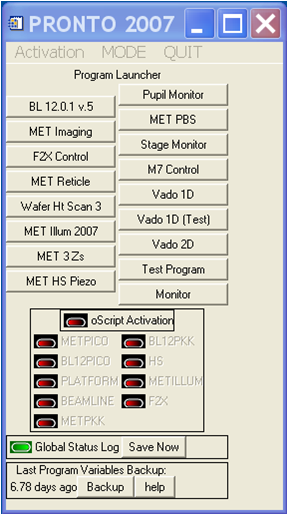
\includegraphics[scale=0.5]{img/met3-pronto.png}
			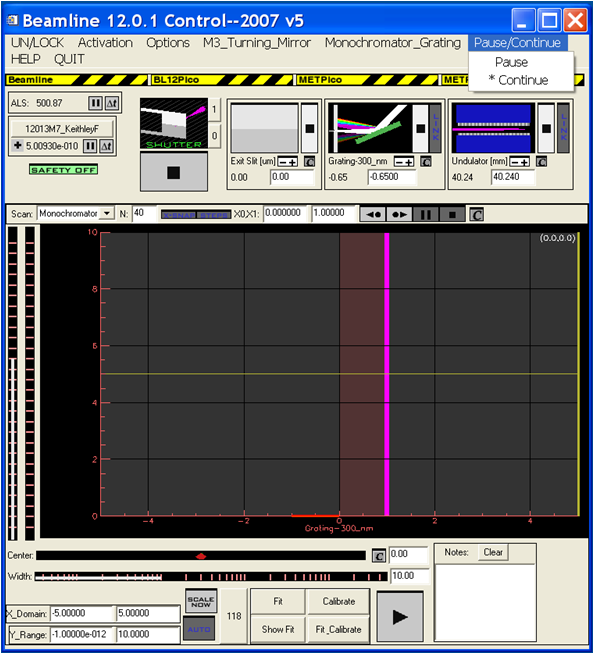
\includegraphics[scale=0.5]{img/met3-beamline.png}
			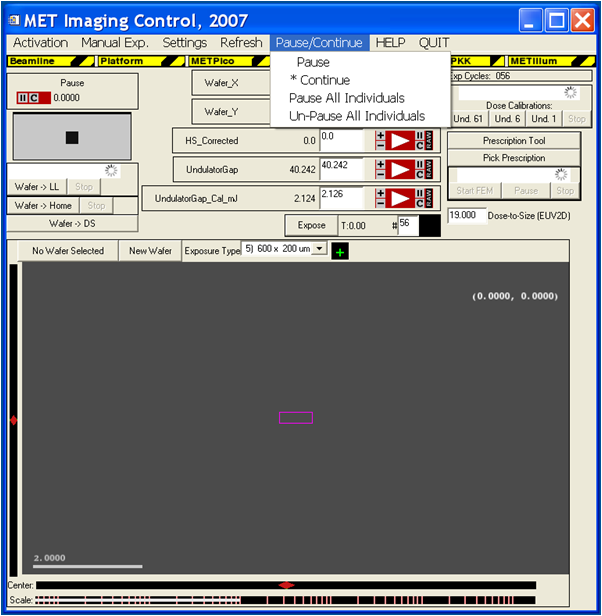
\includegraphics[scale=0.5]{img/met3-imaging.png}}
			\centerline{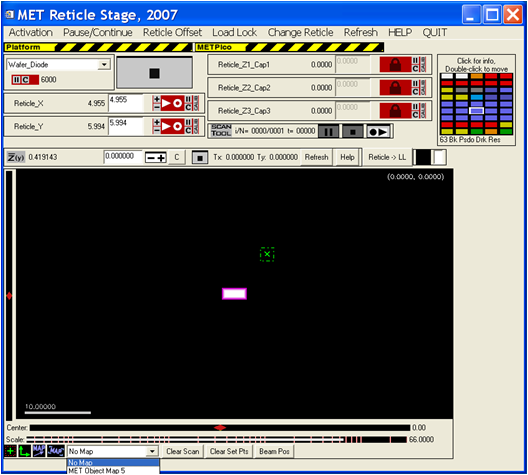
\includegraphics[scale=0.5]{img/met3-reticle.png}
			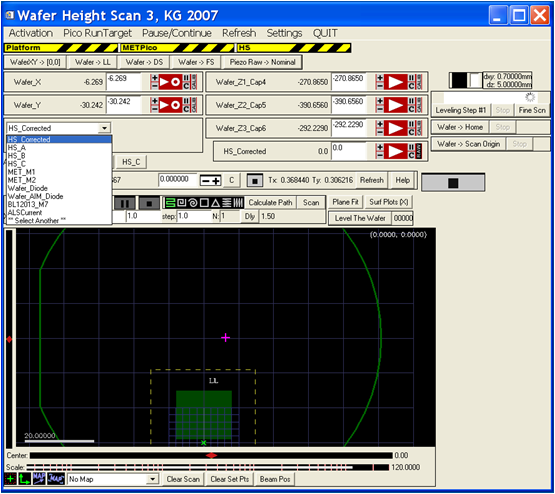
\includegraphics[scale=0.5]{img/met3-wafer.png}
			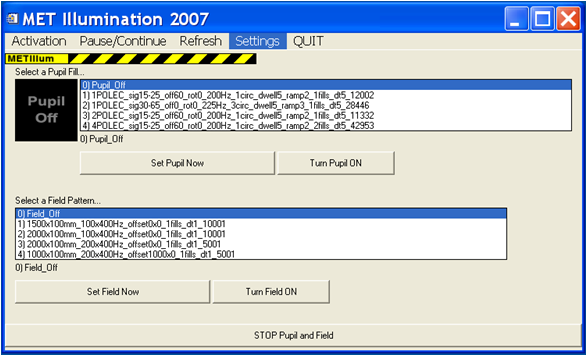
\includegraphics[scale=0.5]{img/met3-illumination.png}}
			\caption{MET3 sotware GUI (courtesy of Ken Goldberg.)}
			\label{fig:met3-elements}
			\end{figure}
			It has been made thoroughly tested and debugged. 
			It is worth mentionning that the soft consistently crashes when it has not been reinitialized after one day, for not obvious reasons.
		
			\subsubsection{SHARP}
			The latest software designed by Ken Goldberg benefited from all the previous tool software development experience. 
			The main improvement was the creation of the concept of \textit{Chaperon}, 
			which is a global thread manager that allow the gracious synchronization of all the elements of the software, which are divided into many chunks to increase the scalability of the code (Fig \ref{fig:sharp-breakdown}).
			
			\begin{figure}[!ht]
			\centerline{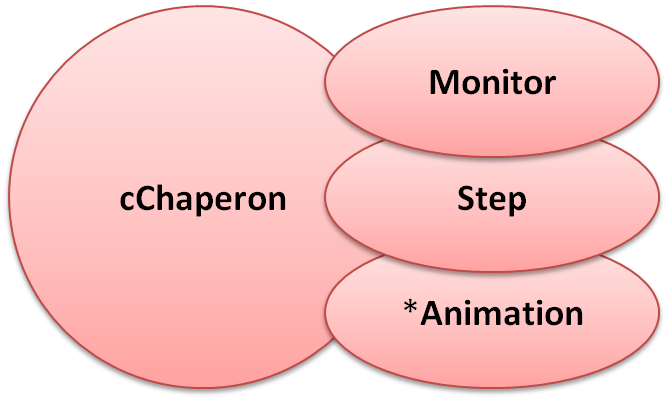
\includegraphics[scale=0.5]{img/sharp-chaperon.png}}
			\centerline{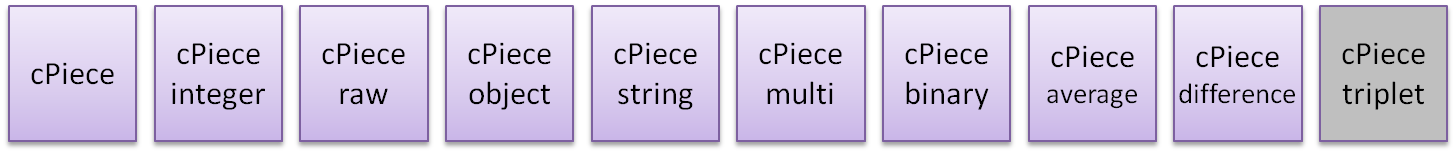
\includegraphics[scale=0.3]{img/sharp-pieces.png}}
			\centerline{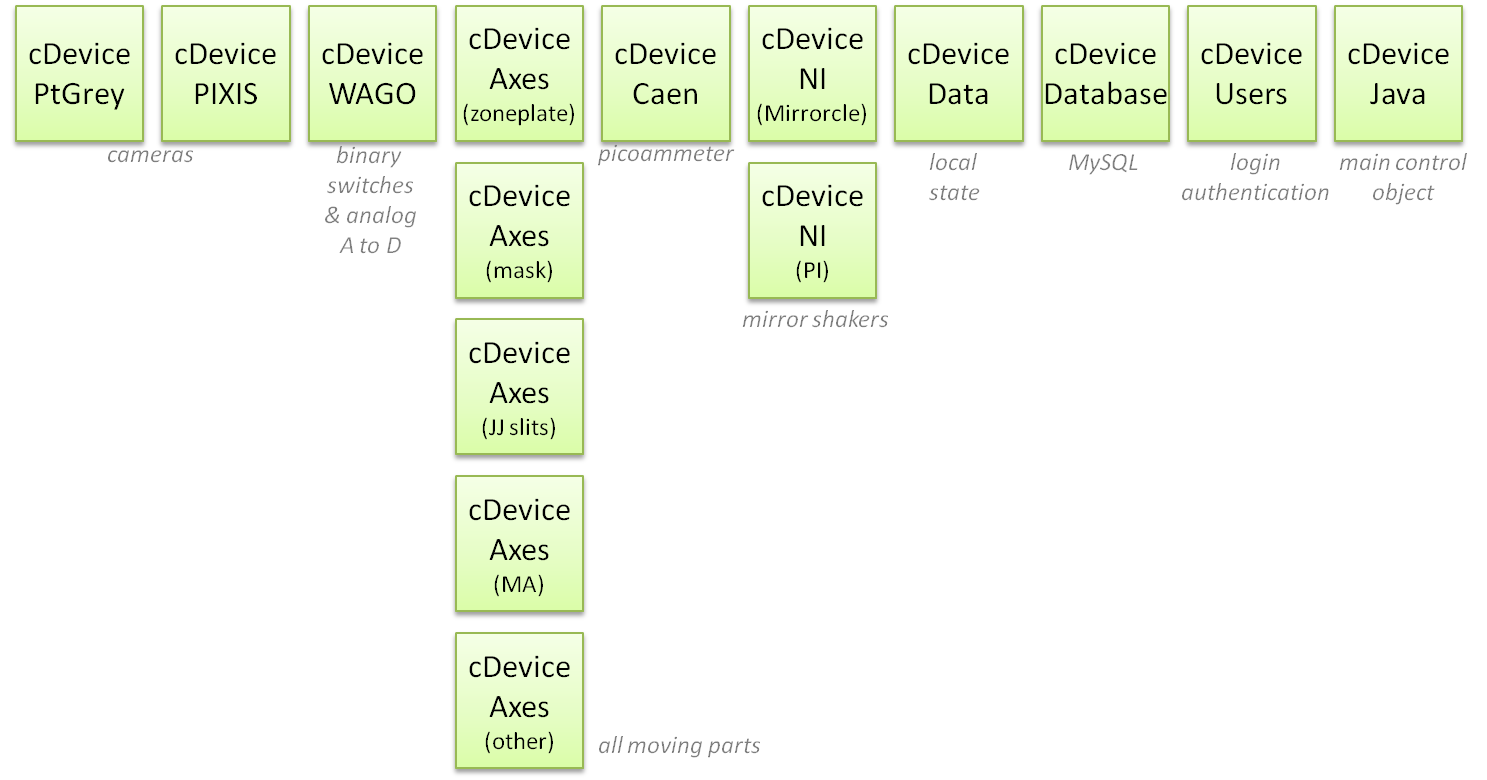
\includegraphics[scale=0.3]{img/sharp-objects.png}}
			\caption{SHARP software structure breakdown (courtesy of Ken Goldberg.)}
			\label{fig:sharp-breakdown}
			\end{figure}
			
			In addition, the UX was carefully designed, especially for the keyboard navigation increasing ease-of-use for the users of the tool 			(Fig.~\ref{fig:sharp-axis}).
			\begin{figure}[!ht]
			\centerline{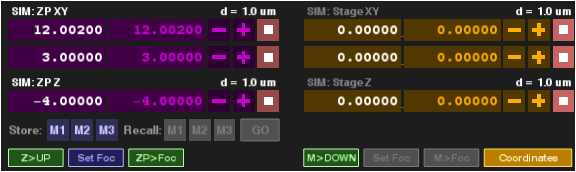
\includegraphics[scale=0.5]{img/sharp-axis.png}}
			\caption{SHARP axis control}
			\label{fig:sharp-axis}
			\end{figure}
			\subsubsection{Pupil Fill Monitor}
			The CXRO Pupil Fill Monitor (PFM) software was developed by Chris Anderson using \textsc{Matlab} (Fig.~\ref{fig:met3-pupil}.) 
			
			\begin{figure}[!ht]
			\centerline{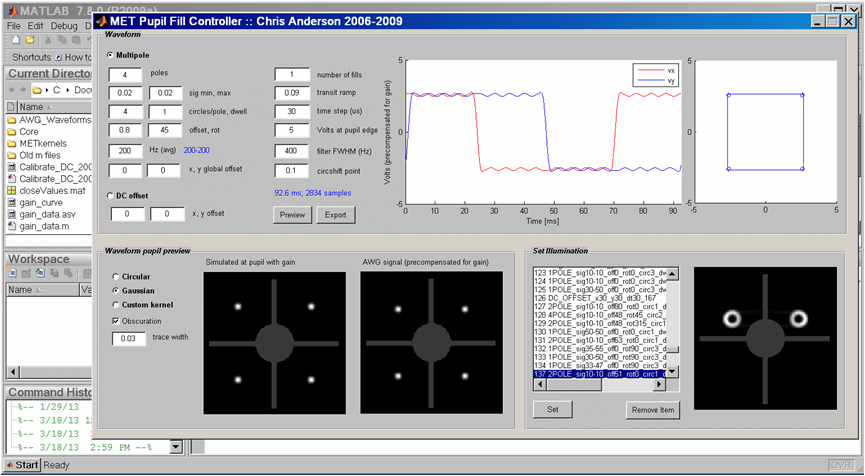
\includegraphics[scale=0.5]{img/met3-pupil.png}}
			\caption{CXRO Pupil Fill Monitor GUI.}
			\label{fig:met3-pupil}
			\end{figure}
			It served as a proof-of-concept validation, and helped to lay the foundation of met3gui.

	\vfill
	\clearpage
	\section{User experience}
	We wanted to leverage the user experience (UX) of users of the current MET3 tool, in order to produce the. 
	We interviewed MET3 operators, who told us they were happy with the current software, especially its modular aspect \comment{a transcipt of the interviews is available somewhere}, and they had no particular grief to tell us. 
	This is why we tried to keep the met5gui structure as similar as possible to MET3 software.
	
	\subsection{Standardizing API for Matlab}
			Since there is no framework in \textsc{Matlab} to perform measurements, we have defined a standard that all met5gui components should follow.
		
	\subsubsection{Vital components}
	\label{sec:vital}
			In this framework, the most vital functions are :
			
			\begin{itemize}
			\item \textbf{Move} defined as absolute and in raw units,
			\item \textbf{Read position/sensor} defined as absolute and in raw units,
			\item \textbf{Completed Motion} $\simeq$ \verb!isThere! to check motion completion,
			\item \textbf{Abort} to stop/abort the current motion (change in target or emergency stop),			
			\end{itemize}

			
			\subsection{Matlab class breakdown}
			Most of met5gui classes must have these methods :
			\begin{itemize}
			\item \textbf{constructor}
			creates an instance of a class; it must not include vital elements such has motor initialization, which are refactored in the \verb!init! method,
			\item \textbf{init}
			initializes the instruments, loads the libraries etc. It is decoupled from the constructor in order to allow for re-initialization,
			\item \textbf{build}
			builds the UI element corresponding to the class (controls and windows).
			\item \textbf{handleClock}
			defines what are the actions to perform when the class is called by the common clock,
			\item \textbf{delete}
			frees the memory gracefully.\\
			Even if there is a garbage collector in \textsc{Matlab}, things can go awry if the class is not isolated from the rest of the elements before it is deleted (the object must be removed from the clock task list, UI elements must be killed, all members that are instances of of controller class must be disconnected and deleted);			
			\end{itemize}
	
\section{History}
It is certainly interesting to recall the decisions and why we have made them.
\subsection{The choice of Matlab}
We have favored \textsc{Matlab} over \textsc{Java} and \verb!C++! for versatility and stability.
The use of an interpreted language is 

\textsc{Java} would have been interesting for it is ubiquitous and could be ported to any kind of device (computer, tablet or even smartphone), and could have been good for connectivity purposes (e.g. communicating data through a website). 
However, some stability issues and the lack of powerful tools for scientific computing to lead us dismiss this choice.

\textsc{Python} was overlooked, for it is not the first choice for a robust GUI. Available Framework (such as \textsc{SciPy} or \textsc{PyQT}) could have been a good help for scientific computing.
\verb!C++! is a compiled language, but the fact that the bytecode imposes an extreme dependence on the choice of the machine the code runs on would impose problems on deployment of the software solution.

MET3's software and SHARP demonstrated that a high level language would work well for the purpose of controlling a lithography tool. 
That is, \textsc{Matlab} being agile with both \verb!C++! DLL and \textsc{Java} classes and somehow platform-independent, added to the fact that newer version of \textsc{Matlab} allows Object-Oriented Programming easy to debug, to build robust Graphical User Interface and that it can be compiled and easily deployed without the actual need for a license, it turned out to be the best choice for MET5 software development.

\subsection{Controllers in \textsc{Java}}
At the very beginning, we had to choose whether the low-level components would be coded in \verb!C++! or \textsc{Java}.
A series of test were lead to compare the speed of both solutions, and \textsc{Java} proved to perform well. 
It also has the advantage of being somehow more compliant with \textsc{Corba} or \textsc{Ice}. 
Many in-house low-level controllers have already been coded using \textsc{Java}, hence empowering us to leverage on already available controllers.
The 32~bits vs. 64~bits problem also seems to be less relevant in the case of \textsc{Java}, so we eventually decided to use this programming language for hardware control.

A solution using \textsc{Matlab} MEX files was dismissed, for they do not allow the keep the hand on the hardware at all time \comment{it this really true ?}.

\subsection{Initial Timeline}
The initial schedule for met5gui is presented Fig.\ref{fig:timeline}.
\begin{figure}[ht]
	\centerline{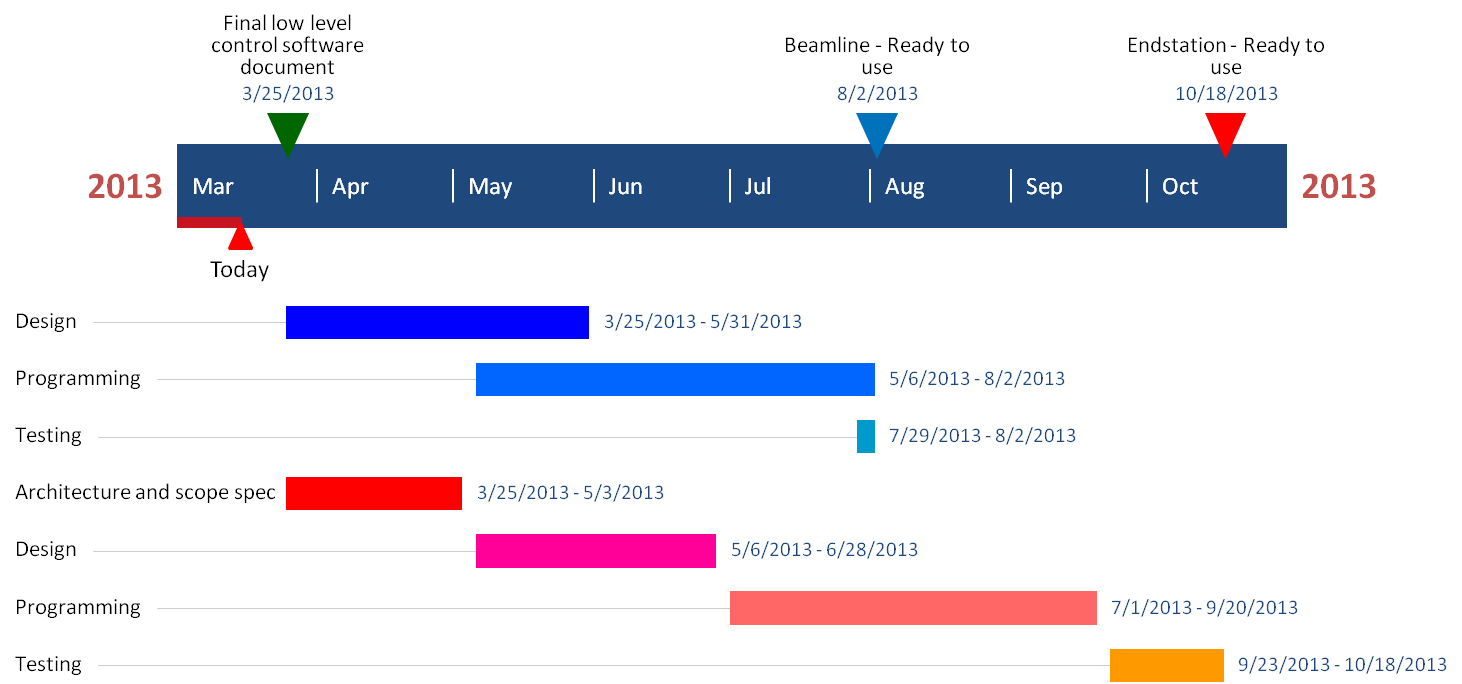
\includegraphics[width=\textwidth]{img/schedule.png}}
	\caption{Initial project timeline, as defined March 15$^{\mbox{th}}$, 2013}
	\label{fig:timeline}
\end{figure}
This schedule was defined at a time when the beamline components were believed to be delivered by August 2013, and the MET5 end-station ready to use by mid-October 2013. As of November 2013, the project is not completed. Most of the components are ready, and deploying is believed to be relatively easy.

The met5gui infrastructure has not been tested on the actual system for obvious reasons. 
Yet, it has been thoroughly debugged, tested and validated on several experiments presented in section \ref{sec:roe}, and we believe that adapting to the lithography tool and fine-tuning should be straightforward, given that all the lower-level elements are operative (motors, cables, controllers, DLL \& \textsc{Java} classes).

\section{System integration}
met5gui is a on top of many elements, and it is legitimate to questions whether some desirable system features, such as kinematics calculations or closed-loop action, can be delegated to lower layers. The actual communication route via \textsc{VMI} or \textsc{CORBA} must also be discussed.

\subsection{EPS and kill switches}
All the EPS and kill switches should be low level, to prevent any malfunction in the software.
However, some 'security' features such as camera can be implemented at higher level, for they require an action from the users.

\subsection{Feedback loops}
Feedback loops, essential to keep the wafer at level by compensating for drifts, must defined at low level, since they need to operate at high speed (1~KHz).
Moreover, having feedback loops at different levels of the system might be detrimental, for that might cause interferences between loops acting at different levels.

\subsection{Compound measurements}
In the case of compound measurements, \textit{i.e.} measurements that are aggregated into a single value, like the height of the height sensor, it would be preferable to have the calculations done at lower level, since these value are meant to feed feedback loop, which might be disturbed by too much overhead in the software.

However, since these measurements rely on calibration (\textsc{e.g.} the actual spot size on each segmented diode, or a best-fit), having the compound measurements at higher level can be beneficial. Though, the main software could easily interact with lower-level controllers to perform calibration.

\subsection{Kinematics}
The kinematics could be handled by the software, though some stage kinematics algorithm might be proprietary and provided by the vendors, like in the case of an Hexapod.
For simpler systems (\textsc{e.g.} wafer stage, Z-Tip-Tilt), we might envision to use the software to perform these calculations.

Again, the need to operate a feedback loop at high-speed might drive the need to have these algorithms implemented at low-level, though it might be helpful to have control on the the kinematics algorithm to correct errors in calibration, \textsc{e.g.} imperfect parallelism between stages.

\subsection{Major shifts}
The major shifts we've made during the process of developing met5gui are the following :
\subsubsection{Hungarian notation}
\textsc{Matlab} performing loose enforcement on data types, we decided to use the Hungarian notation to prevent obfuscation in the code. 
\subsection{Wrapping UIElements}
To comply with the requirement for separation between data and interface, we decided to create UI elements that perform basic data validation and can be easily abstracted form the data.
\subsubsection{Save \& load}
To save the state of the tool, we decided to implement a recursive procedure, so that the parameters can be (re-)loaded by a simple function call.
\subsection{A Clock to rule them all}
The discussion we had with Ken Goldberg about SHARP software, and the difficulties we had to synchronize all the timers included in many different classes, lead us to the creation of a class, \verb!Clock!, inspireed by SHARP's \textit{Chaperon} that is shared by most of the other classes, defining a clear sequence for the actions to be performed. 
We had issues with speed at first, that were corrected by tuning memory allocation.
\subsubsection{Separation of Axis and HardwareIO}
Using the met5gui framework on other experiments, it became clear that there is a fundamental difference between the motion of a stage (performed using \verb!HardwareIO!) and the motion of an object in space(\textit{e.g.} along a direction, perfomed using \verb!Axis!), which can be a compound motion.


\subsection{Return of experiment} \label{sec:roe}
During the course of programming for met5gui, many experiments were led in the optical prototyping room.
Since most wrappers were non-existent or wildly out-of-date, it was required to write all the \textsc{Matlab} from scratch, leveraging on-the-spot training, knowledge and available experience.
That is, it was a good occasion to put at use the met5gui framework, debugging its features, extending its possibilities and questioning its functions.
Here is what we've learned from building acquisition tools :

\subsubsection{AIS}
Building the optical prototype for \emph{AIS} required to write from many stage control and sensor classes, including a flexure stage and diode controlled by a \textit{PaulBox}, a set of two \textit{Micronix} VT50 linear stages using a \textsc{Galil} controller, and a Z-Tip-Tilt tripod developed in-house.
\subsubsection{Z-tip-tilt tripod}
The Z-tip-tilt tripod developed at CXRO is meant to provide increased stiffness in the Z-direction compared to other tripod structures.
It comprises three \textit{Micronix} Pp30-8MM stick-slip translation stage, whose motions are transferred to a main platform (Fig.~\ref{fig:tripod})
\begin{figure}[ht]
	\centerline{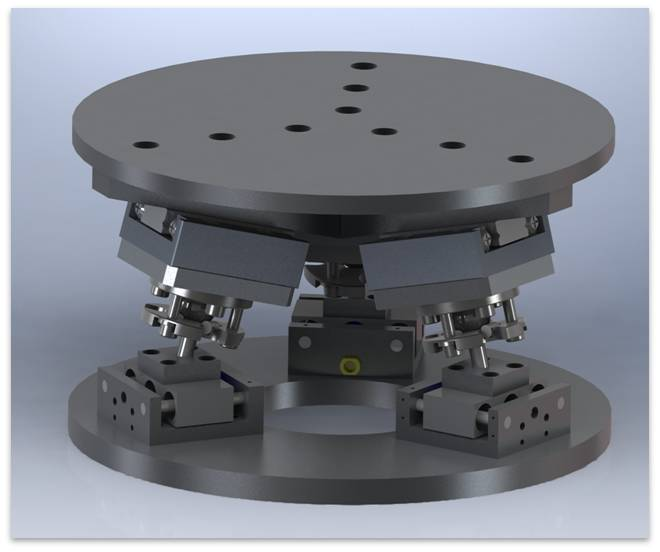
\includegraphics[height=2in]{img/tripod_3d.jpg}
	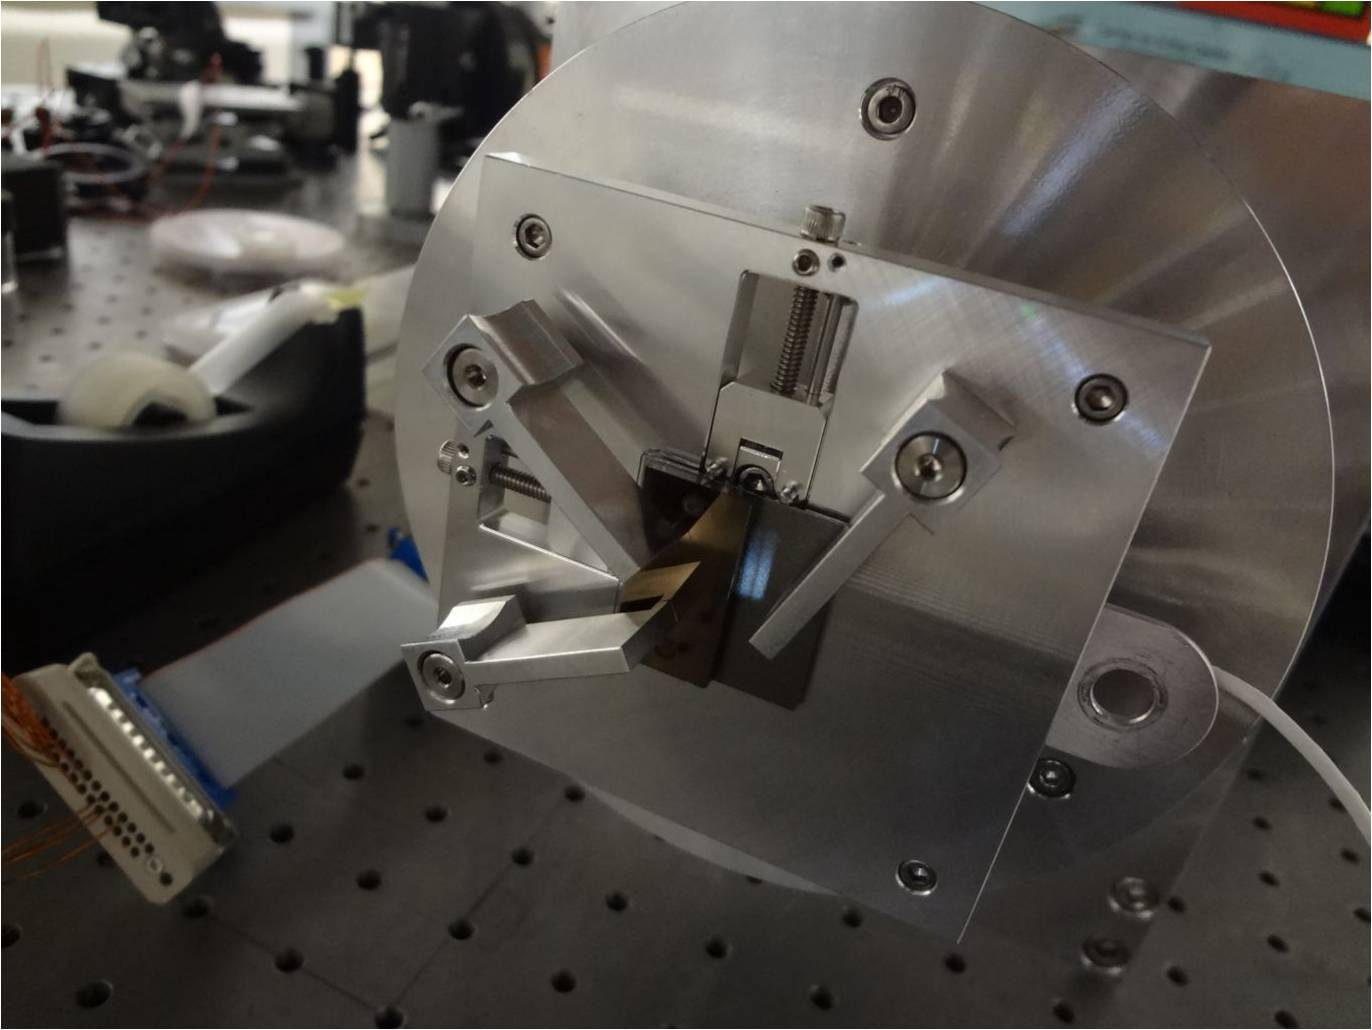
\includegraphics[height=2in]{img/tripod_mounted.jpg}}
	\caption{CXRO's Z-Tip-Tilt tripod. 	left : 3D CAD model -- right : mounted tripod in the AIS experiment.}
	\label{fig:tripod}
\end{figure}
The kinematics relations were not defined yet; we managed to figure them out, and allow a user to independently change the height, the tip and the tilt, by abstracting individual motors position \textit{(a detailed report is available upon request.)}
This lead us to separate the notion of \verb!Axis! and \verb!HardwareIO! in the met5gui framework (Fig.~\ref{fig:exp}, left). 

The AIS Experiment also gave us some feedback to carve out a coherent stage and sensor framework : the flexure stage is actuated through a \verb!C++! DLL, the VT50 linear stage directly through a \textsc{Java} class, while the tripod uses a \textsc{Java} class to communicate with the stage, allowing to send queries to the individual motor.

At the end of it, \emph{AIS} experimental results were found satisfactory.

\subsubsection{Coded Aperture}
The \emph{coded aperture} experiment taught us how to deal with other kinds of motors and sensors, slightly different~: a XZ two-axis stage coupled to an optical encoder through a \textsc{Galil} controller and a photo-diode whose output was read through a \textsc{Wago} ADC.
It was a good occasion to interact with Carl Cork and get a mutual better understanding of what were our needs and our issues, and become aware of certain subtleties such as the partial incompatibility of \textsc{Java} versions 1.6 and 1.7 (only one can be loaded with \textsc{Matlab}), but also Operating Systems incompatibilities with some drivers (some drivers do not work on \textit{Windows 7}.)

The alignment of the setup required the use of a camera, what was the starting point for programming the \verb!Camera! class.
With all the fine-tuning allowed by the use of a coherent framework (not really met5gui yet), \emph{coded aperture} experimental results were deemed suitable for publication.

\subsubsection{Picomotors and cap sensors vacuum test}
Deploying some of the tools created for \emph{AIS} and \emph{coded aperture} experiments on an other setup proved the robustness of a limited subset of the framework (Fig.~\ref{fig:exp}, right), while attracting the attention on the fact that \textsc{Matlab} versions are not fully compatible. 
However, newest iterations of the language seems to be pretty solid.

\subsubsection{Coherent Multiplexed Ptychography}
The current study of \emph{Coherent Multiplexed Ptychography} allowed us to try stage motion, coupled with camera acquisition and asynchronous scanning procedure (the first real-life test for the \verb!Scan! class.)

\begin{figure}[ht]
	\centerline{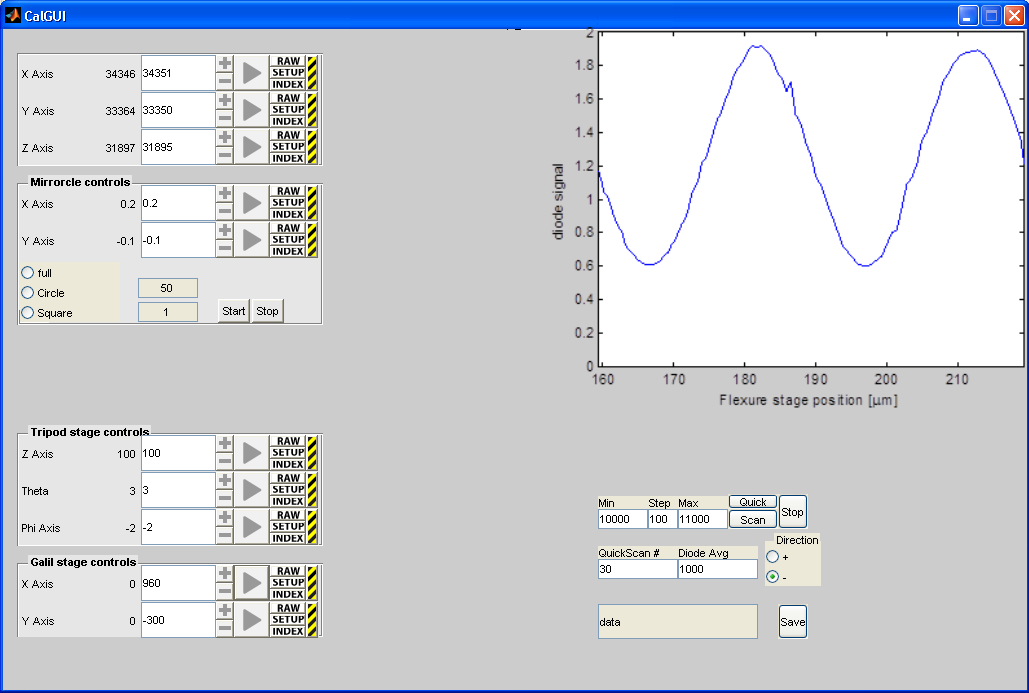
\includegraphics[height=2in]{img/exp-calGUI.png}
	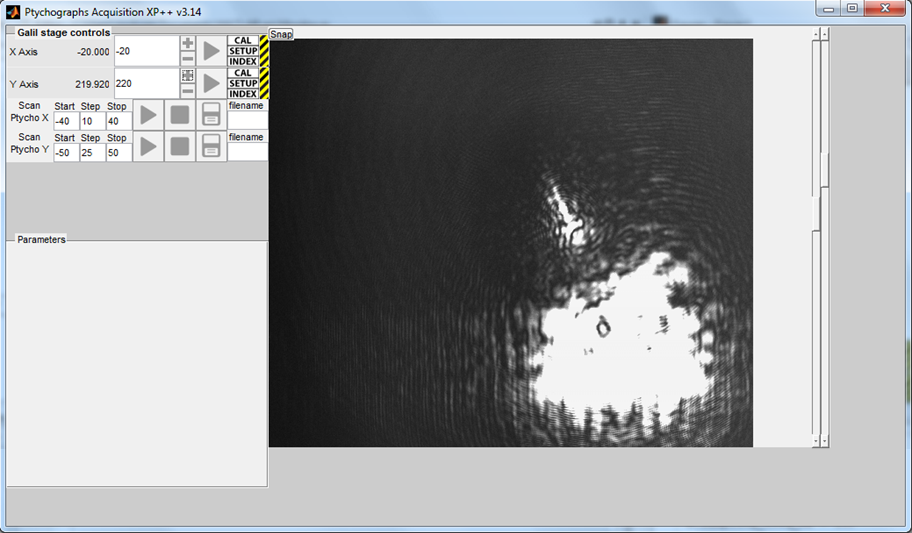
\includegraphics[height=2in]{img/exp-ptycho.png}}
	\caption{Examples of two UIs based on met5gui. left : CalGUI (\textit{AIS}) -- right : Ptychography Acquisition.}
	\label{fig:exp}
\end{figure}

\chapter{Implementation \& Conventions}
\section{Software structure}
\temp{needs further developments}

\section{Naming conventions}
met5gui follows both \textit{CamelCase} notation (\textit{e.g.} \verb!nameOfMyVariable!) and \textit{Hungarian} notation, \textit{i.e.} the name a of a variable is prefixed by the data type (\textit{e.g.} a string is prefixed with a c, like \verb!cMyString!). Properties of a class which are objects have a two letter prefix, \textit{e.g.} an \verb!AxisStetup! property within an \verb!Axis! class will be named \verb!asSetup!. 

Underscores must be avoided (they conflict with the \textit{CamelCase} notation), except in the case a property that has a dimension, which (ideally) should be suffixed (\textit{e.g.} \verb!currentWavelength_nm!).

\section{Matlab compliance}
To allow for a unrestricted class capabilities, all of our classes inherit from the \textsc{Matlab} \verb!handle! class. 
Further, all the classes inherit from a custom \verb!HandlePlus! class which has a few saving and load methods added to the \verb!handle! class.

\chapter{Documentation}
We provide here a description of the main components of met5gui.

\section{Clock}
\verb!Clock! is the class that coordinates all the actions of the other classes.
It is shared by most of the components to allow for an asynchronous operation, \textit{i.e.} to avoid blocking procedures.
It registers all the actions that are automated, such as reading updates or scanning procedures.
It also allows the user to pause the program, making it easier to troubleshoot specific components.

\section{Instrument control}
\subsection{Axis}
\!Axis! is the class that 
It has the capability to operate in a raw or calibrated mode (set through \verb!AxisSetup!), and provides simulation mode through a virtual axis \verb!AxisVirtual!.
It is different from \verb!HardwareIO! in the sense that it doesn't command the position of an actual motor, rather the position of an object.
Typically, the position input will be fed to a low-level kinematics algorithm, or to a bunch of (undisplayed) \verb!HardwareIO! classes working together to produce the required movement.\\
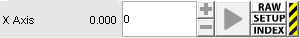
\includegraphics[scale=1]{img/met5gui-Axis.png}
\subsubsection{AxisSetup}
It allows for changing the settings of the \verb!Axis! class display.\\
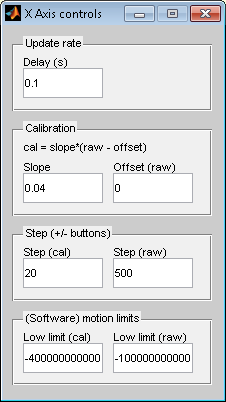
\includegraphics[scale=0.5]{img/met5gui-AxisSetup.png}
\subsubsection{AxisWithSave}
\temp{what are the specifics of this class?}
\subsubsection{AxisAPI}
It is a template class to show the capability of \verb!Axis! to perform of compound movement\\
(\textit{i.e.} it contains the kinematic transforms.)
\subsubsection{AxisAPITest}
Provides the binding between \verb!Axis! and the stage, when the stage has the generic methods listed in section~\ref{sec:vital}.\\
\temp{deprecated, used in AIS, will be turned into APIGeneric }
\subsubsection{AxisVirtual}
Simulates the behavior of a motor for testing purposes.

\subsection{Diode}
\!Diode! is the class that communicate with a sensor, pretty much like \verb!Axis! communicates with a motor.
The reading can be a compound of several readings, contrary to \verb!HardwareO!.\\

\includegraphics[scale=1]{img/met5gui-HardwareO.png}
\subsubsection{DiodeSetup}
The equivalent of \verb!AxisSetup!, for a diode.
\subsection{DiodeAPI}
\temp{There is no such class yet, but there should be one, for general coherence.}
\subsubsection{DiodeVirtual}
The equivalent of \verb!AxisVirtual!, for a diode

\subsection{HardwareIO}
\verb!HardwareIO! is the class that has the direct control over a stage.
It is structurally similar to \verb!Axis! class, except that it doesn't allow for compound movements.
\subsubsection{SetupHardwareIO}
The equivalent of \verb!AxisSetup!, for a stage motion.
\temp{Why is is called SetupHardwareIO ?}
\subsection{HardwareO}
\verb!HardwareO! completes the same role as \verb!HardwareIO! for \verb!Axis!, but for the \verb!Diode! class.

\subsection{Shutter}
\verb!Shutter! allows to trigger a shutter, \textit{i.e.} it is a countdown countdown timer.\\
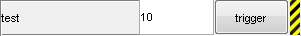
\includegraphics[scale=1]{img/met5gui-Shutter.png}
\subsubsection{ShutterVirtual}
It is a virtual shutter, used for software testing and troubleshooting.

\subsection{Camera}
The \verb!Camera! class establishes the communication with a camera, allowing continuous measurements and snapshots, with the ability to change exposure and gain settings.\\
\temp{It is not fully implemented yet. The \emph{Ptychography} setup currently running serves as an iterator.}

\subsection{Scan}
The \verb!Scan! class allows to scan any number (2D, 3D, 4D, etc.) of any kind of dimension (space (stage), time (shutter), angle, averaging, etc.) in an asynchronous, non-blocking fashion. 
It versatility has been tested through the \verb!ScanTest! class (which comprises many examples of scanning procedure).\\
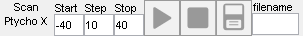
\includegraphics[scale=1]{img/met5gui-Scan.png}

\subsection{Monitor}
The \verb!Monitor! class is pretty much like the scan, but performs continuous measurement in only one dimension (time), pretty much like an oscilloscope. It is very helpful for debugging and troubleshoot procedures, or simply for quick tests performed on a instrument.

\section{API \& wrappers}
\subsection{nPoint}
\temp{to be edited}
\subsection{APIVHardwareIO}
\temp{to be edited}
\subsection{APIHardwareIOnPoint}
\temp{to be edited}
\subsection{ConfigMotor}
\temp{to be edited; what is that, actually?}

\section{UI elements}
All the previous classes uses custom UI elements classes, rather than the \textsc{Matlab} \verb!uicontrol! class, to enforce coherence within the code and performs some extra functions.
\subsection{UIEdit}
It is an editbox that performs data validation and imposes min/max constraints on the entered data.
\subsection{UIButton}
\subsection{UIList}
\subsection{UIText}
\subsection{UICheckbox}
\subsection{UIToggle}
It is similar to a button, but the displayed text/image changes after it is clicked.
\subsection{UIPopup}
\subsection{UI2DNav}
\verb!UI2DNav! allows to pan and zoom an object.
\subsection{List}
\temp{what is that?}
\subsection{Panel}
\temp{what is that ?}
\subsection{Utils}
It is a set of common purpose functions, \textit{e.g.} correcting the user-unfriendly UI elements of \textsc{Matlab} or for allowing scrolling iteration in an editbox.

\section{Controls}
\subsection{Mirror}
This panel is meant to control the beamline mirrors positions.\\
\temp{it is not fully implemented yet, for there still are uncertainties on the low-level controls}

\subsection{ReticlePick}
This is the Reticle Pick of the MET5 software, that allow users to chose among different configuration sets.\\
\subsubsection{ReticlePickPanel}
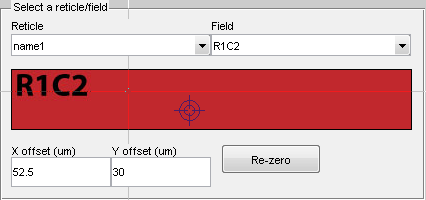
\includegraphics[scale=0.5]{img/met5gui-ReticlePick.png}

\subsection{PupilFill}
This is the control of the Pupil Fill Monitor of MET5.\\
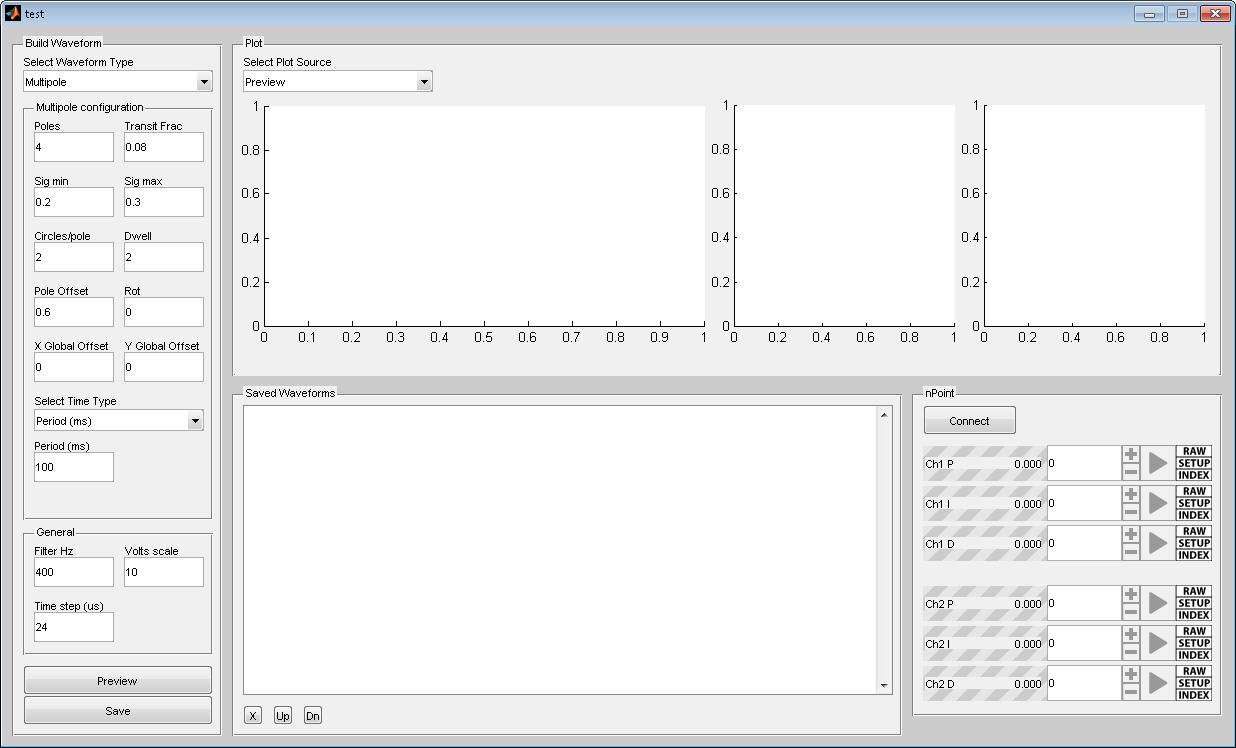
\includegraphics[scale=0.33]{img/met5gui-PupilFill.png}
	\subsubsection{PupilFillCore}

\subsection{HeightSensor}
This is the control of the Height Sensor integrated to MET5.\\
\includegraphics[scale=0.33]{img/met5gui-heightSensor.png}
	\subsubsection{HeightSensorCore}


\section{Debugging and examples}
There are a few classes that were coded to allow for quick debugging and provide examples of how some the elements are meant to be used :
\begin{itemize}
\item Window
\item DemoPanel
\item ClockTest
\item ScanTest
\end{itemize}


\chapter{Room for improvement}
We have successful overcome many of the issues we've face. There are still some (non-critical) issues that haven't tackled yet :
\begin{itemize}
\item When using the clock, the debugging procedure is quite difficult. Adding some verbosity to the process would be a great ,
\item The clock doesn't know ho to handle deleted class (that generally happens when the a class is deleted before the clock),
\item Clock should have an interface that allows to see what is happening in the current cycle, with maybe the ability to slow down the processes and to log and verbose all automated actions,
\item in \verb!UIEDit!, setting the min and max values to $\pm\infty$ is still a problem : Matlab sometimes handles the min/max allowed value symbolically or as number (like \verb!eps!),
\item When a \verb!UIEdit! is edited in a modal window, the user have to validate the choice (by hitting \emph{Enter} or clicking in another box). This is cumbersome, since when the user closes the window, he might have the impression that the edit box has been validated, which might be not,
\item It would be nice to have a fully coherent layout manager (a component would be place at the bottom of another),
\item Keyboard control and general user-friendliness should be improved, and some automation should be implemented (like "go to previous position").
\item the issue of 32 vs. 64~bits controllers has not been carefully examined. It might be a problem if the computers get updated.
\item the issue of \textsc{Java} 1.6 vs. 1.7 has not been solved. Newer versions of \textsc{Matlab use} \textsc{Java} 1.7, but their might be some broken legacy compatibility.
\end{itemize}

\chapter{Annex}
\small \label{sec:annex}
\section{Newport ESP300 controller - 3-axes linear stage controller}
%http://assets.newport.com/webDocuments-EN/images/14293.PDF
\begin{enumerate}
\item AB abort motion 
\item AC set acceleration. 
\item AE set e-stop deceleration 
\item AF set acceleration feed-forward gain. 
\item AG set deceleration. 
\item AP abort program 
\item AU set maximum acceleration and deceleration. 
\item BA set backlash compensation 
\item BG assign DIO bits to execute stored programs 
\item BK assign DIO bits to inhibit motion 
\item BL enable DIO bits to inhibit motion . 
\item BM assign DIO bits to notify motion status. 
\item BN enable DIO bits to notify motion status. 
\item BO set DIO port A, B direction 
\item BP assign DIO bits for jog mode 
\item BQ enable DIO bits for jog mode 
\item CL set closed loop update interval. 
\item CO set linear compensation 
\item DB set position deadband. 
\item DC setup data acquisition 
\item DD get data acquisition done status 
\item DE enable/disable data acquisition  
\item DF get data acquisition sample count 
\item DG get acquisition data . 
\item DH define home. 
\item DL define label 
\item DO set dac offset  
\item DP read desired position. 
\item DV read desired velocity. 
\item EO automatic execution on power on. 
\item EP enter program mode 
\item ES define event action command string. 
\item EX execute a program 
\item FE set maximum following error threshold 
\item FP set position display resolution. 
\item FR set encoder full-step resolution 
\item GR set master-slave reduction ratio  
\item HA set group acceleration  
\item HB read list of groups assigned 
\item HC move group along an arc 
\item xii PrefaceHD set group deceleration 
\item HE set group e-stop deceleration  
\item HF group off. 
\item HJ set group jerk. 
\item HL move group along a line 
\item HN create new group. 
\item HO group on 
\item HP read group position  
\item HQ wait for group command buffer level 
\item HS stop group motion 
\item HV set group velocity 
\item HW wait for group motion stop. 
\item HX delete group 
\item HZ read group size 
\item ID read stage model and serial number. 
\item JH set jog high speed 
\item JK set jerk rate 
\item JL jump to label . 
\item JW set jog low speed 
\item KD set derivative gain. 
\item KI set integral gain 
\item KP set proportional gain  
\item KS set saturation level of integral factor. 
\item LP list program 
\item MD read motion done status 
\item MF motor off. 
\item MO motor on 
\item MT move to hardware travel limit. 
\item MV move indefinitely 
\item MZ move to nearest index  
\item OH set home search high speed. 
\item OL set home search low speed 
\item OM set home search mode 
\item OR search for home 
\item PA move to absolute position . 
\item PH get hardware status. 
\item PR move to relative position 
\item QD update motor driversettings 
\item QG set gear constant 
\item QI set maximum motor current 
\item QM set motor type. 
\item QP quit program mode 
\item QR reduce motor torque. 
\item QS set microstep factor 
\item QT set tachometer gain  
\item QV set average motor voltage . 
\item Preface xiii RS reset the controller 
\item SB set / get DIO port A, B bit status. 
\item SI set master-slave jog velocity update interval 
\item SK set master-slave jog velocity scaling coefficients 
\item SL set left travel limit. 
\item SM save settings to non-volatile memory  
\item SN set axis displacement units 
\item SR set right travel limit 
\item SS define master-slave relationship  
\item ST stop motion. 
\item SU set encoder resolution  
\item TB read error message . 
\item TE read error code . 
\item TJ set trajectory mode. 
\item TP read actual position 
\item TS read controller status 
\item TV read actual velocity 
\item TX read controller activity. 
\item UF update servo filter. 
\item UH wait for DIO bit high. 
\item UL wait for DIO bit low 
\item VA set velocity 
\item VB set base velocity for step motors 
\item VE read controller firmware version 
\item VF set velocity feed-forward gain . 
\item VU set maximum velocity 
\item WP wait for position 
\item WS wait for motion stop 
\item WT wait  
\item XM read available memory. 
\item XX erase program 
\item ZA set amplifier I/O configuration. 
\item ZB set feedback configuration. 
\item ZE set e-stop configuration. 
\item ZF set following error configuration 
\item ZH set hardware limit configuration 
\item ZS set software limit configuration 
\item ZU get ESP system configuration 
\item ZZ set system configuration 
\end{enumerate}


\section{SmarAct MCS 3-Axes Piezo motor controller}
%http://www.trioptics.fr/fichiers/produits/fichiers/MCSProgrammersGuide_v1.6.pdf
\begin{itemize}
\item GetDLLVersion. 
\item GetAvailableSystems 
\item AddSystemToInitSystemsList 
\item ClearInitSystemsList. 
\item InitSystems 
\item ReleaseSystems 
\item GetNumberOfSystems. 
\item GetSystemID 
\item GetNumberOfChannels 
\item GetChannelType 
\item SetHCMEnabled. 
\item Functions for Synchronous Communication. 
\begin{enumerate}
\item SetClosedLoopMaxFrequency 
\item SetClosedLoopMoveSpeed 
\item GetClosedLoopMoveSpeed 
\item SetPosition. 
\item SetZeroPosition 
\item GetPhysicalPositionKnown 
\item SetPositionLimit. 
\item GetPositionLimit. 
\item SetAngleLimit. 
\item GetAngleLimit. 
\item SetStepWhileScan. 
\item SetSensorEnabled. 
\item GetSensorEnabled. 
\item SetSensorType. 
\item GetSensorType. 
\item SetAccumulateRelativePositions 
\item SetEndEffectorType. 
\item GetEndEffectorType. 
\item SetZeroForce 
\item StepMove. 
\item ScanMoveAbsolute. 
\item ScanMoveRelative. 
\item GotoPositionAbsolute 
\item GotoPositionRelative 
\item GotoAngleAbsolute 
\item GotoAngleRelative 
\item Stop 
\item CalibrateSensor 
\item FindReferenceMark 
\item GotoGripperOpeningAbsolute. 
\item GotoGripperOpeningRelative. 
\item GotoGripperForceAbsolute 
\item GetVoltageLevel 
\item GetPosition. 
\item GetAngle. 
\item GetStatus 
\item GetGripperOpening 
\item GetForce 
\end{enumerate}
\item Functions for Asynchronous Communication 
\begin{enumerate}
\item GetClosedLoopMoveSpeed 
\item GetPhysicalPositionKnown 
\item GetPositionLimit. 
\item GetAngleLimit. 
\item SetReportOnComplete 
\item GetSensorEnabled. 
\item GetSensorType. 
\item GetEndEffectorType. 
\item GetVoltageLevel 
\item GetPosition. 
\item GetAngle. 
\item GetStatus 
\item GetGripperOpening 
\item GetForce. 
\item SetReceiveNotification 
\item ReceiveNextPacket 
\item ReceiveNextPacketIfChannel. 
\item LookAtNextPacket. 
\item DiscardPacket.
\end{enumerate}
\end{itemize}



\section{Stanford Research Systems SR830 DSP Lock-In Amplifier}
%http://www.thinksrs.com/downloads/PDFs/Manuals/SR830m.pdf
\begin{enumerate}
\item OUTX i The SR830 OUTX i command sets the output interface to RS232 (i=0) or GPIB (i=1). 
\item FMOD i The SR530 is always in external reference mode. 
\item AX AY AR The AX, AY and AR commands auto offset the X, Y and R outputs.  
\item AP The AP command performs the Auto Phase function. 
\item B {n} The SR830 has no bandpass filter. 
\item C {n} Changes the Reference display. 
\item D {n} Change the dynamic reserve. Unlike the SR530, all reserves are allowed at all sensitivities. 
\item E m {,n} Change the Channel m expand. n=2 selects expand by 100. 
\item F {x} The F command Reads the frequency.
\item G {n} Change the sensitivity from 10 nV (n=1) to 500 mV (n=24).
\item I {n} Change the remote/local status. The SR830 Override Remote mode can override the I2 command.
\item L m {,n} Change the line notch filter status.  
\item M {n} Change the reference mode to 2f. 
\item N {m} Change the noise bandwidth.
\item OX {n} {,v} OY {n} {,v} OR {n} {,v} Change the X, Y or R offsets. 
\item P {v} Change the reference phase shift. The value of v is limited to -360.0=v=729.99.
\item Q1 Q2 QX QY Read the output values in Volts or degrees. 
\item R {n} Change the reference input mode. 
\item S {n} Change the Output displays. 
\item T m {,n} Change the time constant. 
\item V {n} Change the value of the SRQ mask. 
\item X n {,v} Set or query the auxiliary analog ports. 
\item Y {n} Not implemented. Do not use. 
\item Z Reset the SR830. The instrument is reset to the SR830 default setup listed in the Operation section.
\end{enumerate}

\section{GalilAxisVT50}
(from CXRO java controller)
\begin{enumerate}
\item abortMove() 
\item destroy() 
\item disable() 
\item enable() 
\item getAcceleration() 
\item getAuxEncoderOffset() 
\item getAuxEncoderPosition() 
\item getAuxEncoderScale() 
\item getAxisUnits() 
\item getLowerLimitHard() 
\item getLowerLimitSoft() 
\item getName() 
\item getOffset() 
\item getPosition() 
\item getPositionRaw() 
\item getScale() 
\item getSpeed() 
\item getSwitches() 
\item getTarget() 
\item getTargetRaw() 
\item getUpperLimitHard() 
\item getUpperLimitSoft() 
\item hasAuxEncoder() 
\item initialize() 
\item isEnabled() 
\item isInitialized() 
\item isLocked() 
\item isReady() 
\item isStopped() 
\item loadConfigs() 
\item moveAbsolute(double dest) 
\item moveAbsoluteRaw(double destRaw) 
\item moveRelative(double dist) 
\item moveRelativeRaw(double distRaw) 
\item saveConfigs() 
\item setAcceleration(double accel) 
\item setAuxEncoderOffset(double auxEncoderOffset) 
\item setAuxEncoderPosition(double auxEncoderPosition) 
\item setAuxEncoderScale(double auxEncoderScale) 
\item setAxisUnits(java.lang.String axisUnits) 
\item setLowerLimitSoft(double lowerLimit) 
\item setOffset(double offset) 
\item setPosition(double pos) 
\item setScale(double inScale) 
\item setSpeed(double speed) 
\item setTarget(double dest) 
\item setTargetRaw(double rawDest) 
\item setUpperLimitSoft(double upperLimit) 
\item stopMove() 
\item unlock() 
\end{enumerate}

\section{Micos PMC100}
(from .h, wrapped with CXRO java class; uses queries)
\begin{itemize}
\item GetNumDevices(lpNumDevices);-	This function is used to get total number of all types of Performax USB modules connected to the PC.
\item GetProductString(dwNumDevices, lpDeviceString,  dwOptions); This function is used to get the Performax product string.  This function is used to find out Performax USB module product string and its associated index number.  Index number starts from 0.
\item ComOpen(dwDeviceNum, pHandle); This function is used to open communication with the Performax USB module and to get communication handle.  Index number starts from 0.  
\item ComClose(pHandle); This function is used to close communication with the Performax USB module.  
\item ComSetTimeouts(dwReadTimeout, DWORD dwWriteTimeout); This function is used to set the communication read and write timeout.  Values are in milliseconds.
\item ComSendRecv(pHandle, wBuffer, dwNumBytesToWrite,dwNumBytesToRead,rBuffer); This function is used to send command and get reply.  Number of bytes to read and write must be 64 characters.
\begin{enumerate}
\item ABORT	Immediately stops the motor if in motion.  For decelerate stop, use STOP command.  This command is used for clearing the StepNLoop error status.
\item ACC	Returns current acceleration value in milliseconds.
\item ACC=[Value]	Sets acceleration value in milliseconds.
\item DN	Returns 4 character device ID.  
\item DN=[Value]	Sets 4 character device ID.  
\item DO	Returns driver general purpose output status	1 – motor power enabled 0 – motor power disabled	0	1
\item DO=[0 or 1]	Enables (value 1) or disables (value 0) general purpose digital output		0	1
\item EO	Returns driver power enable	1 – motor power enabled0 – motor power disabled	0	1
\item EO=[0 or 1]	Enables (value 1) or disables (value 0) motor power		0	1
\item EX	Returns current encoder counter value	Position value in 32 bit 		
\item EX=[value]	Sets the current encoder counter value			
\item HSPD	Returns High Speed Setting	Value in pps	1	6M
\item HSPD=[Value] 	Sets High Speed.		1	6M
\item H+	Homes the motor in positive direction			
\item H-	Homes the motor in negative direction			
\item ID	Return product ID. 	PerformaxUSB-EX		
\item J+	Jogs the motor in positive direction			
\item J-	Jogs the motor in negative direction			
\item LSPD	Returns Low Speed Setting	Value in pps	1	6M
\item LSPD=[Value] 	Sets Low Speed		1	6M
\item LT=[0 or 1]	Enable or disable position latch feature			
\item LTE	Returns latched encoder position	Encoder position		
\item LTP	Returns latched pulse position	Pulse position		
\item LTS	Returns latch status.	0 – Latch off 1 – Latch on and waiting for latch trigger 2 – Latch triggered.		
\item MST	Returns motor status	Bit 0 – constant speed Bit 1 – accelerating Bit 2 – decelerating ...
\item POL	Returns current polarity	Bit 0 - Pulse Bit 1 - Dir  ..
\item POL=[value]	Sets polarity.			
\item PS	Returns current pulse speed			
\item PX	Returns current position value	Position value in 32 bit 		
\item PX=[value]	Sets the current position value			
\item SCV	Returns the s-curve control	0 or 1	0	1
\item SCV=[0 or 1]	Enable or disable s-curve.  If disabled, trapezoidal acceleration/deceleration will be used.			
\item SL	Returns StepNLoop control status	0 – StepNLoop Off  1 – StepNLoop On		
\item SL=[0 or 1]	Enable or disable StepNLoop control			
\item SLA	Returns maximum number of StepNLoop control attempt			
\item SLA=[value]	Sets maximum number of StepNLoop control attempt		1	16
\item SLE	Returns StepNLoop correction value.			
\item SLE=[value]	Sets StepNLoop correction value.			
\item SLR	Returns StepNLoop ratio value			
\item SLR=[factor]	Sets StepNLoop ratio value.  			
\item SLS	Returns current status of StepNLoop control	-1 – Not applicable  0 – Idle  1 – Moving ...
\item SLT	Returns StepNLoop tolerance value			
\item SLT=[value]	Sets StepNLoop tolerance value.  			
\item SSPD[Value]	Performax on-the-fly speed change.  
\item STOP	Decelerates to stop the motor if in motion.  For immediate stop, use ABORT command.			
\item VER	Returns current firmware software version number	Vxxx		
\item X[value]	Moves the motor to absolute position value using the HSPD, LSPD, and ACC values. Maximum allowed incremental move amount is 262143. 
\item ZH+	Homes the motor in positive direction using the home switch and then Z index encoder channel.			
\item ZH-	Homes the motor in negative direction using the home switch and then Z index encoder channel.			
\end{enumerate}
\end{itemize}


\section{Mirrorcle}
(from CXRO's DLL header file)
\begin{enumerate}
\item Uninit(unsigned long phandle);
\item Init(unsigned long phandle, uint id, float Vmaxin);
\item SendDataStream(unsigned long handle, float* x, float* y, float* dout, int len, int sps, uint loop);
\item GoToXY(unsigned long handle, float x, float y);
\item EnableAmplifier(unsigned long handle, uint state);
\item StartDataStream(unsigned long handle);
\item StopDataStream(unsigned long handle);
\item AbortDataStream(unsigned long handle);
\item ClearDataStream(unsigned long handle, int sps);
\item Home(unsigned long handle);
\item IsInitialized(unsigned long handle);
\end{enumerate}

\section{Wago}
(from CXRO's java wrapper)
\begin{enumerate}
\item connect
\item disconnect
\item gettAllInputs
\item getSingleInput
\end{enumerate}

\section{PaulBox}
(from CXRO's DLL header file)
\begin{enumerate}
\item init(void);
\item beepTest(long iCount);
\item attach(int, char *argv[]);
\item deattach(void);
\item serverStatus(void);
\item startServer(void);
\item killServer(void);
\item motorMoveto(long box, long mot, long goal);
\item motorLock(long box, long mot, long goal);
\item motorUnlock(long box, long mot);
\item motorRun(long box, long mot, long dir, long sp);
\item motorStop(long box);
\item stopAll();
\item motorAbort(long box);
\item abortAll();
\item motorGetPos(long box, long mot);
\item motorReadPos(long box, long mot);
\item sensorGet(long box, long sens);
\item sensorRead(long box, long sens);
\item getState(long box);
\item getPort(long box);
\item getTol(long box, long mot, long delay);
\item getLim(long box, long mot, long high);
\item getTun(long box, long mot, long wx);
\item getPol(long box, long mot);
\item getFil(long wx);
\item getUpdate();
\item getAvg(long box, long mot);
\item getSensorAvg(long box, long sens);
\item getContUpd();
\item getSmrFlag();
\item getActiveMotor(long box, long mot);
\item getLockedMotor(long box, long mot);
\item getActiveVoltage(long box, long sensor);
\item setUpdate(long update);
\item setPort(long box, unsigned short int port);
\item setTol(long box, long mot, long tol, long delay);
\item setLim(long box, long mot, long low, long high);
\item setTun(long box, long mot, long w1, long w2, ...);
\item setPol(long box, long mot, long pol);
\item setFil(long f1, long f2, long f3, long f4);
\item setAvg(long box, long mot, long avg);
\item setSensorAvg(long box, long sens, long avg);
\item setContUpd(long f1);
\item setSmrFlag(long f1);
\item setActiveMotor(long box, long mot, bool value);
\item setActiveVoltage(long box, long sensor, bool value);
\item autoTun(long box, long mot, long method);
\item autoPol(long box, long mot);
\end{enumerate}


\end{document}
